% Practice Test 13 — Maryland Edition
% Questions: 30 (18 MC + 12 SA)
% Generated by scripts/generate_practice_tests.py

\begin{practiceQuestion}{1-3-q16}{mc}
\begin{questionText}
A map uses a scale where $1$ cm represents $25$ km. What is the constant of proportionality in km per cm?
\end{questionText}
\choiceA{$0.04$}
\choiceB{$1$}
\choiceC{$25$}
\choiceD{$250$}
\correctAnswer{C}
\explanation{$k = \frac{25 \text{ km}}{1 \text{ cm}} = 25$ km per cm.}
\end{practiceQuestion}

\begin{practiceQuestion}{1-5-q18}{mc}
\begin{questionText}
A store sells oranges. The graph passes through $(6, 4.50)$. What is the cost of $10$ oranges?
\end{questionText}
\choiceA{$\$6.50$}
\choiceB{$\$7.00$}
\choiceC{$\$7.50$}
\choiceD{$\$10.50$}
\correctAnswer{C}
\explanation{$k = \frac{4.50}{6} = 0.75$. Cost of $10$: $0.75 \times 10 = \$7.50$.}
\end{practiceQuestion}

\begin{practiceQuestion}{1-6-q14}{mc}
\begin{questionText}
A school orders $240$ lunches for $320$ students. At the same rate, how many lunches should they order for $400$ students?
\end{questionText}
\choiceA{$280$}
\choiceB{$300$}
\choiceC{$320$}
\choiceD{$360$}
\correctAnswer{B}
\explanation{$\frac{240}{320} = \frac{x}{400}$. Cross-multiply: $320x = 96{,}000$, so $x = 300$ lunches.}
\end{practiceQuestion}

\begin{practiceQuestion}{2-1-q19}{sa}
\begin{questionText}
What is $65\%$ of $140$?
\end{questionText}
\correctAnswer{$91$}
\explanation{$65\% = 0.65$. Multiply: $0.65 \times 140 = 91$.}
\end{practiceQuestion}

\begin{practiceQuestion}{2-5-q30}{gsa}
\begin{questionText}
The bar graph shows the monthly sales for a salesperson over $4$ months. She earns $6\%$ commission. What is her total commission for all $4$ months?

\begin{center}
\begin{tikzpicture}[scale=0.5]
  \draw[thick,->] (0,0) -- (0,7) node[above]{\small Sales (\$)};
  \draw[thick,->] (0,0) -- (9.5,0);
  \fill[funBlue!60] (0.5,0) rectangle (1.5,4);
  \fill[funBlue!60] (2.5,0) rectangle (3.5,5);
  \fill[funBlue!60] (4.5,0) rectangle (5.5,3);
  \fill[funBlue!60] (6.5,0) rectangle (7.5,6);
  \node[below,font=\small] at (1,0) {Jan};
  \node[below,font=\small] at (3,0) {Feb};
  \node[below,font=\small] at (5,0) {Mar};
  \node[below,font=\small] at (7,0) {Apr};
  \foreach \y/\lab in {2/4000,4/8000,6/12000} {
    \draw (-0.1,\y) -- (0.1,\y) node[left,font=\small,xshift=-2pt] {\lab};
  }
  \node[above,font=\small] at (1,4) {$8{,}000$};
  \node[above,font=\small] at (3,5) {$10{,}000$};
  \node[above,font=\small] at (5,3) {$6{,}000$};
  \node[above,font=\small] at (7,6) {$12{,}000$};
\end{tikzpicture}
\end{center}
\end{questionText}
\correctAnswer{$\$2{,}160$}
\explanation{Total sales: $8{,}000 + 10{,}000 + 6{,}000 + 12{,}000 = \$36{,}000$. Commission: $36{,}000 \times 0.06 = \$2{,}160$.}
\end{practiceQuestion}

\begin{practiceQuestion}{2-7-q22}{sa}
\begin{questionText}
A lab experiment expected to produce $250$ mL but produced $240$ mL. Find the percent error.
\end{questionText}
\correctAnswer{$\approx 4.2\%$}
\explanation{$\frac{|250 - 240|}{240} \times 100 = \frac{10}{240} \times 100 \approx 4.17 \approx 4.2\%$.}
\end{practiceQuestion}

\begin{practiceQuestion}{3-1-q01}{mc}
\begin{questionText}
What is the opposite of $-6$?
\end{questionText}
\choiceA{$-6$}
\choiceB{$0$}
\choiceC{$6$}
\choiceD{$\frac{1}{6}$}
\correctAnswer{C}
\explanation{The opposite of a negative number is positive. The opposite of $-6$ is $6$ because both are $6$ units from $0$.}
\end{practiceQuestion}

\begin{practiceQuestion}{3-2-q15}{mc}
\begin{questionText}
What is $(-25) + 13 + (-8)$?
\end{questionText}
\choiceA{$-20$}
\choiceB{$-46$}
\choiceC{$30$}
\choiceD{$-4$}
\correctAnswer{A}
\explanation{$(-25) + 13 = -12$. Then $(-12) + (-8) = -20$.}
\end{practiceQuestion}

\begin{practiceQuestion}{4-1-q21}{sa}
\begin{questionText}
A pool is being filled at a rate of $8$ gallons per minute. It already has $50$ gallons of water. Write an expression for the amount of water after $t$ minutes, then find the amount after $15$ minutes.
\end{questionText}
\correctAnswer{$8t + 50$; $170$ gallons}
\explanation{The expression is $8t + 50$. Substitute $t = 15$: $8(15) + 50 = 120 + 50 = 170$ gallons.}
\end{practiceQuestion}

\begin{practiceQuestion}{4-2-q26}{gmc}
\begin{questionText}
The algebra tiles below represent an expression. Which is the simplified form?

\begin{center}
\begin{tikzpicture}[scale=0.55]
  % Positive x-tiles
  \fill[funBlue!40] (0,0) rectangle (2,1);
  \draw[thick] (0,0) rectangle (2,1);
  \node at (1,0.5) {$x$};
  \fill[funBlue!40] (2.3,0) rectangle (4.3,1);
  \draw[thick] (2.3,0) rectangle (4.3,1);
  \node at (3.3,0.5) {$x$};
  \fill[funBlue!40] (4.6,0) rectangle (6.6,1);
  \draw[thick] (4.6,0) rectangle (6.6,1);
  \node at (5.6,0.5) {$x$};
  \fill[funBlue!40] (6.9,0) rectangle (8.9,1);
  \draw[thick] (6.9,0) rectangle (8.9,1);
  \node at (7.9,0.5) {$x$};
  \fill[funBlue!40] (9.2,0) rectangle (11.2,1);
  \draw[thick] (9.2,0) rectangle (11.2,1);
  \node at (10.2,0.5) {$x$};
  % Negative x-tiles
  \fill[funRed!40] (0,-1.5) rectangle (2,-0.5);
  \draw[thick] (0,-1.5) rectangle (2,-0.5);
  \node at (1,-1) {$-x$};
  \fill[funRed!40] (2.3,-1.5) rectangle (4.3,-0.5);
  \draw[thick] (2.3,-1.5) rectangle (4.3,-0.5);
  \node at (3.3,-1) {$-x$};
  % Positive unit tiles
  \fill[funGreen!40] (6,-1.5) rectangle (7,-0.5);
  \draw[thick] (6,-1.5) rectangle (7,-0.5);
  \node at (6.5,-1) {$1$};
  \fill[funGreen!40] (7.3,-1.5) rectangle (8.3,-0.5);
  \draw[thick] (7.3,-1.5) rectangle (8.3,-0.5);
  \node at (7.8,-1) {$1$};
  \fill[funGreen!40] (8.6,-1.5) rectangle (9.6,-0.5);
  \draw[thick] (8.6,-1.5) rectangle (9.6,-0.5);
  \node at (9.1,-1) {$1$};
  \fill[funGreen!40] (9.9,-1.5) rectangle (10.9,-0.5);
  \draw[thick] (9.9,-1.5) rectangle (10.9,-0.5);
  \node at (10.4,-1) {$1$};
\end{tikzpicture}
\end{center}
\end{questionText}
\choiceA{$5x + 4$}
\choiceB{$3x + 4$}
\choiceC{$7x + 4$}
\choiceD{$3x - 4$}
\correctAnswer{B}
\explanation{There are $5$ positive $x$-tiles and $2$ negative $x$-tiles: $5x + (-2x) = 3x$. There are $4$ positive unit tiles: $+4$. Simplified: $3x + 4$.}
\end{practiceQuestion}

\begin{practiceQuestion}{5-2-q06}{mc}
\begin{questionText}
What is the first step to solve $7x - 3 = 25$?
\end{questionText}
\choiceA{Divide both sides by $7$}
\choiceB{Subtract $3$ from both sides}
\choiceC{Add $3$ to both sides}
\choiceD{Multiply both sides by $7$}
\correctAnswer{C}
\explanation{To undo the subtraction of $3$, add $3$ to both sides first: $7x = 28$.}
\end{practiceQuestion}

\begin{practiceQuestion}{5-3-q20}{sa}
\begin{questionText}
Solve $-6(n - 2) = 42$.
\end{questionText}
\correctAnswer{$n = -5$}
\explanation{Divide by $-6$: $n - 2 = -7$. Add $2$: $n = -5$. Check: $-6(-5 - 2) = -6(-7) = 42$ \checkmark.}
\end{practiceQuestion}

\begin{practiceQuestion}{5-4-q16}{mc}
\begin{questionText}
A student estimates that the solution to $0.48x + 3.1 = 12.7$ is about $x = 20$. Is this estimate reasonable?
\end{questionText}
\choiceA{Yes, the exact answer is $20$}
\choiceB{Yes, the exact answer is close to $20$}
\choiceC{No, the exact answer is about $10$}
\choiceD{No, the exact answer is about $33$}
\correctAnswer{A}
\explanation{Subtract $3.1$: $0.48x = 9.6$. Divide by $0.48$: $x = 20$. The estimate is exactly correct.}
\end{practiceQuestion}

\begin{practiceQuestion}{5-5-q08}{mc}
\begin{questionText}
Solve $\dfrac{x}{3} + 4 < 10$.
\end{questionText}
\choiceA{$x < 18$}
\choiceB{$x < 42$}
\choiceC{$x < 2$}
\choiceD{$x < 6$}
\correctAnswer{A}
\explanation{Subtract $4$: $\frac{x}{3} < 6$. Multiply by $3$: $x < 18$.}
\end{practiceQuestion}

\begin{practiceQuestion}{5-6-q23}{sa}
\begin{questionText}
A phone battery is at $85\%$ and loses $7\%$ per hour. Write an inequality for when the battery is below $20\%$, and solve.
\end{questionText}
\correctAnswer{$85 - 7h < 20$; $h > 9\dfrac{2}{7}$ hours (about $9.3$ hours)}
\explanation{$85 - 7h < 20$. Subtract $85$: $-7h < -65$. Divide by $-7$ and flip: $h > \frac{65}{7} = 9\frac{2}{7}$.}
\end{practiceQuestion}

\begin{practiceQuestion}{6-2-q12}{mc}
\begin{questionText}
A map uses $1$ cm $= 30$ km. A second map uses $1$ cm $= 15$ km. A river is $4.5$ cm long on the first map. How long is it on the second map?
\end{questionText}
\choiceA{$2.25$ cm}
\choiceB{$9$ cm}
\choiceC{$15$ cm}
\choiceD{$67.5$ cm}
\correctAnswer{B}
\explanation{Scale ratio: $\frac{30}{15} = 2$. New length: $4.5 \times 2 = 9$ cm.}
\end{practiceQuestion}

\begin{practiceQuestion}{6-3-q09}{mc}
\begin{questionText}
Can a triangle have sides $2$, $5$, and $2$?
\end{questionText}
\choiceA{Yes, it is an isosceles triangle}
\choiceB{Yes, it is a scalene triangle}
\choiceC{No, because two sides are equal}
\choiceD{No, because $2 + 2 < 5$}
\correctAnswer{D}
\explanation{$2 + 2 = 4 < 5$. The two shorter sides cannot reach across the longest side, so no triangle is possible.}
\end{practiceQuestion}

\begin{practiceQuestion}{6-4-q14}{mc}
\begin{questionText}
Sides $5$, $12$, $13$. Is this a right triangle?
\end{questionText}
\choiceA{No, because $5 + 12 \neq 13$}
\choiceB{No, because the sides are not equal}
\choiceC{Yes, because $5^2 + 12^2 = 13^2$}
\choiceD{Yes, because $5 + 12 = 17 > 13$}
\correctAnswer{C}
\explanation{$5^2 + 12^2 = 25 + 144 = 169 = 13^2$. The Pythagorean theorem holds, so it is a right triangle.}
\end{practiceQuestion}

\begin{practiceQuestion}{6-5-q27}{gmc}
\begin{questionText}
The diagram shows a cone being sliced. Which cut produces a circular cross-section?

\begin{center}
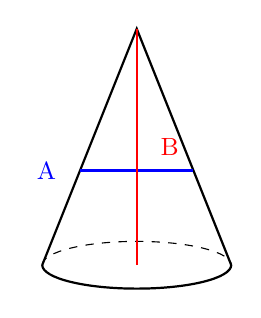
\begin{tikzpicture}[scale=0.6]
  % Cone
  \draw[thick] (-2,0) -- (0,5) -- (2,0);
  \draw[thick] (-2,0) arc[start angle=180,end angle=360,x radius=2,y radius=0.5];
  \draw[dashed] (-2,0) arc[start angle=180,end angle=0,x radius=2,y radius=0.5];
  % Cut A - horizontal
  \draw[thick,blue] (-1.2,2) -- (1.2,2);
  \node[left,blue] at (-1.5,2) {\small A};
  % Cut B - vertical through apex
  \draw[thick,red] (0,0) -- (0,5);
  \node[right,red] at (0.3,2.5) {\small B};
\end{tikzpicture}
\end{center}
\end{questionText}
\choiceA{Cut A (horizontal)}
\choiceB{Cut B (vertical through apex)}
\choiceC{Both cuts}
\choiceD{Neither cut}
\correctAnswer{A}
\explanation{Cut A (horizontal, parallel to the base) produces a circle. Cut B (vertical through the apex) produces a triangle.}
\end{practiceQuestion}

\begin{practiceQuestion}{7-3-q08}{mc}
\begin{questionText}
A circle has an area of $50.24$ m$^2$. Using $\pi \approx 3.14$, what is the diameter?
\end{questionText}
\choiceA{$4$ m}
\choiceB{$8$ m}
\choiceC{$16$ m}
\choiceD{$2$ m}
\correctAnswer{B}
\explanation{$r^2 = 50.24 \div 3.14 = 16$. So $r = 4$ m and $d = 8$ m.}
\end{practiceQuestion}

\begin{practiceQuestion}{7-4-q20}{sa}
\begin{questionText}
A figure is a rectangle $15$ m by $8$ m with a rectangular hole $5$ m by $3$ m cut out. What is the area of the remaining figure?
\end{questionText}
\correctAnswer{$105$ m$^2$}
\explanation{Outer: $15 \times 8 = 120$ m$^2$. Hole: $5 \times 3 = 15$ m$^2$. Remaining: $120 - 15 = 105$ m$^2$.}
\end{practiceQuestion}

\begin{practiceQuestion}{7-5-q19}{sa}
\begin{questionText}
Find the surface area of a rectangular prism with length $8$ cm, width $5$ cm, and height $3$ cm.
\end{questionText}
\correctAnswer{$158$ cm$^2$}
\explanation{$SA = 2(8 \times 5) + 2(8 \times 3) + 2(5 \times 3) = 80 + 48 + 30 = 158$ cm$^2$.}
\end{practiceQuestion}

\begin{practiceQuestion}{7-6-q29}{gsa}
\begin{questionText}
A composite solid is made of two rectangular prisms joined together as shown. What is the total volume?

\begin{center}
\begin{tikzpicture}[scale=0.35]
  % Bottom prism
  \draw[thick,funBlue,fill=funBlue!10] (0,0) rectangle (10,3);
  \draw[thick,funBlue,fill=funBlue!20] (10,0) -- (13,2) -- (13,5) -- (10,3) -- cycle;
  \draw[thick,funBlue,fill=funBlue!15] (0,3) -- (3,5) -- (13,5) -- (10,3) -- cycle;
  % Top prism
  \draw[thick,funRed,fill=funRed!10] (0,3) rectangle (4,6);
  \draw[thick,funRed,fill=funRed!20] (4,3) -- (7,5) -- (7,8) -- (4,6) -- cycle;
  \draw[thick,funRed,fill=funRed!15] (0,6) -- (3,8) -- (7,8) -- (4,6) -- cycle;
  % Labels
  \node[below] at (5,0) {$10$ cm};
  \node[left] at (0,1.5) {$3$ cm};
  \node[right] at (13,3.5) {$3$ cm};
  \node[left] at (0,4.5) {$3$ cm};
  \node[above left] at (2,6) {$4$ cm};
  \node[right] at (7,6.5) {$3$ cm};
\end{tikzpicture}
\end{center}
\end{questionText}
\correctAnswer{$126$ cm$^3$}
\explanation{Bottom prism: $10 \times 3 \times 3 = 90$ cm$^3$. Top prism: $4 \times 3 \times 3 = 36$ cm$^3$. Total: $90 + 36 = 126$ cm$^3$.}
\end{practiceQuestion}

\begin{practiceQuestion}{8-1-q23}{sa}
\begin{questionText}
A radio station asks listeners to call in and vote for their favorite song. Explain why this is not a random sample.
\end{questionText}
\correctAnswer{Only listeners who choose to call participate, so it is voluntary and biased}
\explanation{Voluntary response samples are biased because people with strong opinions are more likely to respond.}
\end{practiceQuestion}

\begin{practiceQuestion}{8-3-q15}{mc}
\begin{questionText}
Group X: mean $45$, range $12$. Group Y: mean $52$, range $12$. What can you say about these groups?
\end{questionText}
\choiceA{They have the same center and different spread}
\choiceB{They have different centers and the same spread}
\choiceC{They are identical}
\choiceD{Group X is more spread out}
\correctAnswer{B}
\explanation{The means differ ($45$ vs.\ $52$) but both have the same range ($12$), so they have different centers and similar spread.}
\end{practiceQuestion}

\begin{practiceQuestion}{8-4-q20}{sa}
\begin{questionText}
Data: $8, 10, 12, 14, 16, 18, 20$. Find the IQR.
\end{questionText}
\correctAnswer{$8$}
\explanation{$Q_1 = 10$, $Q_3 = 18$. IQR $= 18 - 10 = 8$.}
\end{practiceQuestion}

\begin{practiceQuestion}{9-1-q24}{sa}
\begin{questionText}
There are $12$ cards numbered $1$ through $12$ in a box. What is the probability of drawing an even number? Write your answer as a fraction in simplest form.
\end{questionText}
\correctAnswer{$\frac{1}{2}$}
\explanation{Even numbers: $2, 4, 6, 8, 10, 12$ — that is $6$ out of $12$. $P = \frac{6}{12} = \frac{1}{2}$.}
\end{practiceQuestion}

\begin{practiceQuestion}{9-4-q18}{mc}
\begin{questionText}
Ben predicts that a coin will land on heads $50\%$ of the time. He flips the coin $20$ times and gets $14$ heads. What should he conclude?
\end{questionText}
\choiceA{The coin is definitely biased}
\choiceB{His model is exactly correct}
\choiceC{The result is somewhat different from the prediction, but $20$ trials is a small sample}
\choiceD{He should change his model to predict $70\%$ heads}
\correctAnswer{C}
\explanation{$\frac{14}{20} = 0.70$ vs. predicted $0.50$. With only $20$ trials, variation is expected. More trials would provide a better comparison.}
\end{practiceQuestion}

\begin{practiceQuestion}{9-6-q28}{gmc}
\begin{questionText}
The table below shows the sample space for spinning two spinners. Spinner 1 has sections $\{1, 2, 3\}$ and Spinner 2 has sections $\{A, B\}$. If each outcome is equally likely, what is the probability of getting an odd number and the letter B?

\begin{center}
\begin{tabular}{|c|c|c|}
\hline
 & \textbf{A} & \textbf{B} \\
\hline
\textbf{1} & $(1,A)$ & \cellcolor{funGreen!20}$(1,B)$ \\
\hline
\textbf{2} & $(2,A)$ & $(2,B)$ \\
\hline
\textbf{3} & $(3,A)$ & \cellcolor{funGreen!20}$(3,B)$ \\
\hline
\end{tabular}
\end{center}
\end{questionText}
\choiceA{$\frac{1}{6}$}
\choiceB{$\frac{2}{6}$}
\choiceC{$\frac{3}{6}$}
\choiceD{$\frac{4}{6}$}
\correctAnswer{B}
\explanation{Odd numbers: $1, 3$. Favorable outcomes: $(1,B)$ and $(3,B)$ — $2$ out of $6$. $P = \frac{2}{6} = \frac{1}{3}$.}
\end{practiceQuestion}

\begin{practiceQuestion}{9-7-q02}{mc}
\begin{questionText}
A coin flip is used to simulate an event with two equally likely outcomes. Which real-world event could it model?
\end{questionText}
\choiceA{The probability of rain ($30\%$ chance)}
\choiceB{Whether a baby is a boy or girl (approximately $50\%$ each)}
\choiceC{Rolling a $6$ on a die}
\choiceD{Drawing a heart from a deck of cards}
\correctAnswer{B}
\explanation{A coin has two equally likely outcomes ($50\%$ each), which matches the approximately $50/50$ chance of a baby being a boy or girl.}
\end{practiceQuestion}
